% Chapter 3

\chapter{Related Work} % Main chapter title

\label{Related Work} % For referencing the chapter elsewhere, use \ref{Chapter1} 

\lhead{Chapter 3. \emph{Related Work}} % This is for the header on each page - perhaps a shortened title

Evolving virtual creatures in a simulation environment first presented 20 years ago by Karl Sims. In this chapter presents valuable related research work in the areas of evolution in virtual but also physical environments. Novelty search has been used in past work to evolve virtual creatures with no success.


\section{Evolution of Virtual-Physical Robots}

Robot controllers can be evolved through evolutionary algorithms on simulated (virtual) robots, although evolutionary methods can be applied to physical~robots~\cite{nolfi1994evolve} as well, when no damage can occur due to exploration of the action space. 

Novel systems, that make use of evolutionary methods to evolve artificial neural networks which can control the morphology of rigid body parts connected with joints, and forces applied to the joint so virtual creatures (fig.~\ref{fig:karlSims}) can be produced~\cite{sims1994evolving} in a physical three dimensional world. Different fitness measures also give the possibility of the evolution of diverse creatures in respect to these measures. This genetic encoding defines a hyperspace of infinite number of possible creatures and behaviors, and when it is searched using optimization techniques like EA, a variety of successful and interesting locomotion strategies emerge, some of which would be difficult to invent or build by human designers.

Evolvable virtual creatures play an important role in computer graphics when the need for natural looking morphologies can save time from designers. While previous work~\cite{lipson2000automatic} ended up with unnatural looking shapes and behaviors due to vast solution space. A system that uses Lindenmayer systems~\cite{hornby2001evolving} (L-systems) as the encoding of an EA for creating virtual creatures. Creatures evolved by this system have hundreds of parts, and the use of an L-system as the encoding resulted in creature morphologies that have a more natural look.

Evolutionary robotics have shown the ability to evolve complex designs which can complete tasks in their native environment are trained for. However, these complex designs do not serve well engineering purposes of EA, whereas these complicated designs are hard to applied or impossible to made in a physical robot. Generative representation used in~\cite{hornby2003generative}, accomplishes to turn the representation into a construction plan which uses simple robot components in a regular way, moving in this way more effective in the design space. As direct encoding schemes have trouble capturing geometrical properties of the problem, generative encodings like CPPNs can be used in order to take advantage of a problem's regularities and symmetries. 

\begin{figure}[t!]
\centering
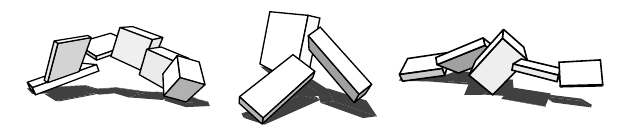
\includegraphics[width=0.8\textwidth]{../Figures/Misc/evolvingVirtualCreatures.png}
\caption{Karl Sims, ``evolution of virtual creatures'' \cite{sims1994evolving}.}
\label{fig:karlSims}
\end{figure}

HyperNEAT~\cite{stanley2009hypercube}, which is a method to evolve CPPNs which will determine the topology and the weights of ANNs, shows promising results in evolving the gaits of legged robots~\cite{clune2009evolving}, where direct encodings have trouble. Natural evolution is the only process which instead that evolving only the brain of biological organisms, it also evolves the morphologies of them. CPPN-NEAT~\cite{stanley2007compositional} can be used as a generative encoding EA which can evolve both features of virtual robots~\cite{auerbach2010dynamic, auerbach2010evolving}, implying that more complex creatures than designers imagination can be created in such a setting. It is also possible that a lower resolution is used at the first runs of the evolution to save computational time without significantly degrading the quality of evolved structures and later a higher resolution for the details optimization.

It has also been shown that evolving objects with encodings based on concepts from biological development like CPPNs can be a powerful way to evolve complex, interesting objects~\cite{clune2011evolving} , which should be of use in fields as diverse as art, engineering, and biology. There is enough evidence as well, that information provided to the CPPNs can also bias the outputs of these networks.

Apart from the use in robot-bodies design evolution, EA techniques coupled with indirect coding schemes allow the evolution of the morphology and the motion control of soft bodies, in this case  multicellular animats~\cite{joachimczak2012co} in a 2-dimensional fluid-like environment. Both the developmental program and motion control are encoded indirectly in a single linear genome, where a genetic algorithm can be applied to evolve it.

With the excel of $3$D printing, soft multi-material robot bodies can actually be produced using simple material types. These soft structures made only by soft materials can be simulated~\cite{hiller2012dynamic} allowing for the evolution of their design without the costs of production. As it is first shown in~\cite{hiller2012automatic}, the automated design of three dimensional bodies which can obtain functionalities through the distribution of hard and soft materials inside the three dimensional space. The robots were evolved (EA) and tested for a single-direction locomotion displacement, whereas it has also been proved, testing a soft material robot inside a pressure-chamber that, the actual error compared to the virtual one in the simulation was small.

\begin{figure}[t!]
\centering
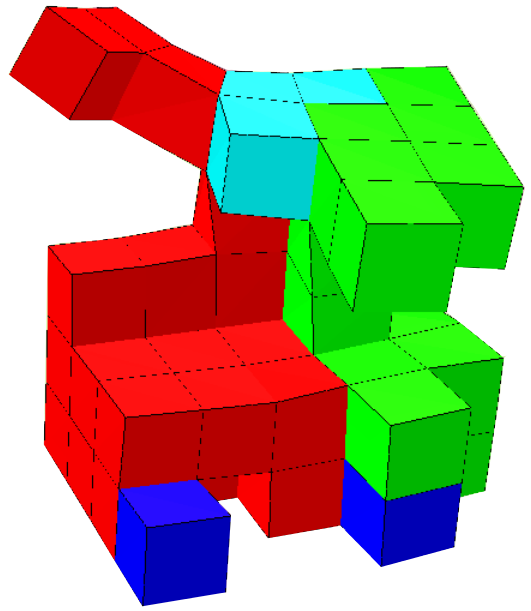
\includegraphics[height=0.2\textwidth]{../Figures/Misc/unshacklingEvolutionFigure1.png}\hspace{0.4cm}
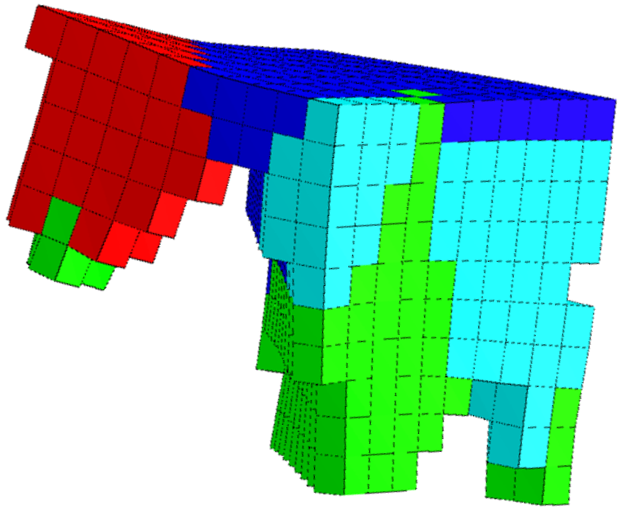
\includegraphics[height=0.2\textwidth]{../Figures/Misc/unshacklingEvolutionFigure2.png}\hspace{0.4cm}
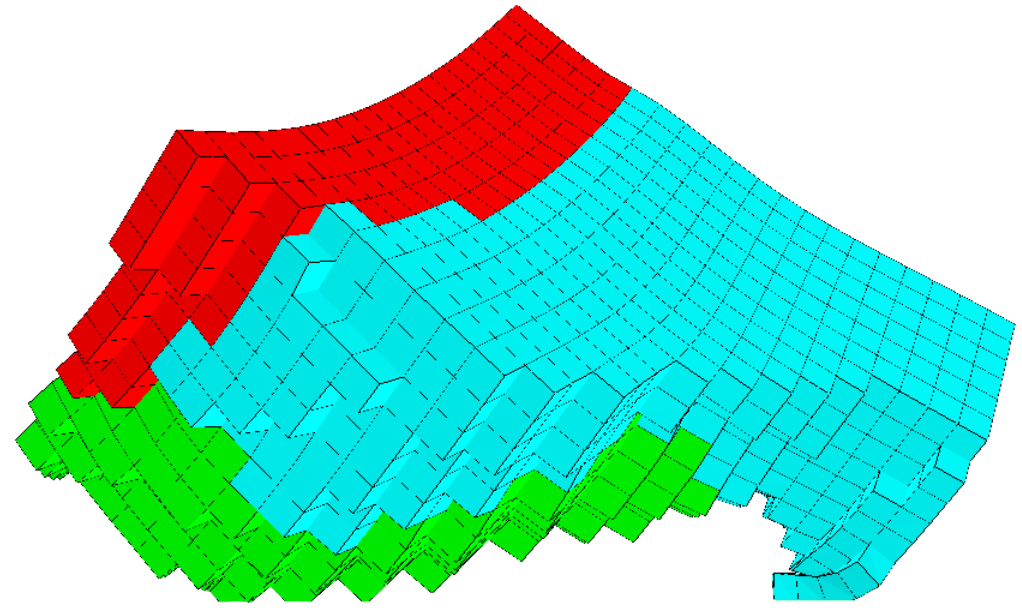
\includegraphics[height=0.2\textwidth]{../Figures/Misc/unshacklingEvolutionFigure3.png}
\caption{Evolution of soft robots' morphology by indirect encoding (CPPN) \cite{cheney2013unshackling}.}
\label{fig:unschackling}
\end{figure}

Evolution of soft material robots as was shown in~\cite{hiller2012automatic} can produce structures able to locomote. The possibility of evolving these soft structures using indirect coding was of interest to be exploited by~\cite{cheney2013unshackling}. A powerful generative encoding, CPPN~\cite{stanley2007compositional}, used to generate soft voxel-formed three dimensional structures (fig.~\ref{fig:unschackling}) like in~\cite{hiller2012automatic}, coupled with the use of NEAT algorithm which ensures the increase of complexity of the networks produced, were purposed for evolving these soft-robots. The superiority of this kind of generative encoding was verified, showing how CPPNs can take advantage of the geometrical properties they show. Evaluation was done by a simple displacement measure. Yet, evolution tended to stick to different kinds of locomotion strategies and morphologies as the fitness function was penalized for different kinds of parameters. Furthermore, it has been shown that evolving morphologies (CPPNs) in lower resolutions and then applying the same networks for higher resolution structures can be beneficial, since the locomotion behaviors in lowers structures apply also in higher, saving in this way computational time.


\section{Evolving Virtual Creatures by Novelty Search}

In problem with such high dimensionality as evolving both the morphology and locomotion strategy of artificial creature in simulated or physical environments, evolution does not explore the solution space enough, sticking only with first easiest to exploit morphologies. However, novelty search, a technique that explicitly rewards diverging, can potentially mitigate such convergence. Methods for evolving such virtual creatures like in~\citep{sims1994evolving}, can utilize novelty search~\citep{lehman2011evolving}, and be far more explorative in the search space. Behavior novelty defined as a measure between morphological properties of the produced creatures driving the evolution to explore more diverse morphologies. This kind of defined behavior cannot led the larger diversity of creatures to move, as different produced morphologies does not guarantee that some of them will actually move. However, combining fitness and novelty metrics through local competition led to improved results, whereas novelty search alone failed. 



\begin{comment}
\section{Evolving gaits}
\todo{Not much idea of what to add here and where I should focus (space?)}
\citep{auerbach2012relationship} On  the  relationship  between  environmental and mechanical complexity in evolved robots.
\citep{lee2013evolving} Evolving gaits  for  physical  robots  with  the  hyperneat  generative  encoding:   The  benefits  of simulation.
\end{comment}

\begin{comment}
\section*{\todo{Additional material that can be added later}}
\citep{clune2011performance}
\citep{clune2013evolutionary}
\citep{lipson2000automatic}
\citep{hiller2010evolving}
\citep{rieffel2014growing}
by tom: \citep{Paoletti07092014}
\end{comment}

